\chapter{Application Controls}
\label{cs:ac}

\section{Controlli di Input}
Quando viene fatta review dei controlli di input, l'auditor deve
assicurare che tutte le transazioni sono state immesse correttamente.
I controlli devono essere in grado di verificare che l'input sia valido.
Questo è molto importante perché in molti sistemi automatizzati,
l'output di un sistema è l'input di un altro. In queste situazioni,
i dati devono essere controllati per verificare le informazioni sia
dalla applicazione mittente che da quella ricevente.

\subsection{Input Form}
Un input form dovrebbe avere le seguenti caratteristiche:
\begin{itemize}
\item Essere facilmente leggibile e utilizzabile;
\item Raggruppare campi simili assieme;
\item Provvedere codici di input predeterminati per ridurre
gli errori;
\item Provvedere identificativi o numeri che fanno riferimento
incrociato ad altri documenti;
\item Indicare la dimensione dei campi;
\item Richiedere firme per l'autorizzazione se necessario.
\end{itemize}

\subsection{Validazione delle Transazioni}
\begin{itemize}
	\item Sequence check: l'utilizzo di sequence number fanno sì che numeri
	out-of-sequence o numeri duplicati vengano rifiutati;
	\item Controllo dell'intervallo e limiti: i numeri sono sotto un numero
	massimo dato o in un intervallo specifico,
	\item Controlli di validità o lookup di una tabella:
	solo alcuni valori sono accettati (es. Sesso = M/F);
	\item Controlli di ragionevolezza: i valori inseriti sono ragionevoli.
	Per esempio per una pizzeria un'ordine di pizza d'asporto di 100 pizze
	va verificato;
	\item Controlli di esistenza: i campi richiesti da compilare
	sono completati correttamente;
	\item Key Verification: l'input è controllato due volte attraverso
	una seconda persona o tutte le cifre sono immesse due volte.
	\item Check Digit: una cifra potrebbe verificare la corretta
	immissione di altre cifre;
	\item Completeness check: viene immesso un input completo. Gli
	spazi o gli zero sono controllati per ogni lettera o cifra
	richiesta;
	\item Duplicate Check: bisogna sempre controllare se una transizione
	con lo stesso ID esiste già. In caso affermativo va rifiutata;
	\item Consistency or Logical Relationship Check: i nuovi dati
	sono coerenti con altri dati a disposizione: per esempio
	la data di nascita di un dipendente deve essere avvenuta almeno
	16 anni fa.
\end{itemize}

Per esempio, oggi come oggi in America hanno poche grandi catene per la pizza.
Questo perché il sistema è diventato informatizzato, garantendo il monopolio a
PizzaHut grazie alla sua applicazione. È per questo che il controllo
sull'input è molto importante, perché un possibile attacco di Denial Of
Service potrebbe essere ordinare un numero incontrollato di pizze.





\subsection{Batch Processing}
È un tipo di controllo dell'input.
Elaborazione sequenziale di blocchi di transazioni
dopo che sono state aggregate.
L'input è autorizzato e raccolto in ``batch''. Vengono effettuati
dei controlli automatici su un batch e associati ad un batch file.
Viene effettuata la validazione delle transazioni. Le transazioni
rifiutate sono corrette e rispedite o trattate in altro modo.

Viene effettuato il processing (es. ordine pagamenti e salvataggio nel DB):
Il processing viene completato.
Infine segue il batch balancing attraverso
una riconciliazione manuale o automatica dei controlli di batch.

Una rappresentazione grafica del batch processing si può trovare in
Figura \ref{fig:security:batch:processing}.
\begin{figure}[h!]
        \begin{center}
                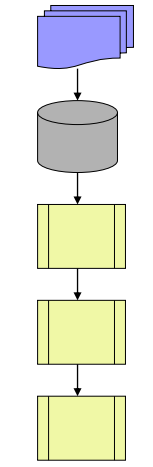
\includegraphics[scale=0.5]{batch_processing}
        \end{center}
        \caption{Batch processing}
        \label{fig:security:batch:processing}
\end{figure}

\subsection{Transaction Authorization}
\begin{itemize}
    \item Manuale: ottenere una firma dal management sui form dei batch o sui
    documenti;
    \item Automatico: controllo online dell'accesso attraverso
    l'identificazione del terminale o della password.
\end{itemize}

\subsection{Alternative per il trattamento degli errori}
Gli errori di input possono essere trattati
con le seguenti tecniche:
\begin{itemize}
\item Rigettare le transazioni con errori e continuare a processare
il batch;
\item Rigettare l'intero batch di transazioni, se contiene
degli errori;
\item Tenere il batch in sospeso fintanto che le transazioni
non vengono fixate;
\item Accettare l'intero batch ma contrassegnare le transazioni che
contengono degli errori per renderne più facile l'identificazione,
permettendo quindi correzioni future.
\end{itemize}






\section{Processing Controls}

\subsection{Data Processing}

\begin{figure}[h!]
        \begin{center}
                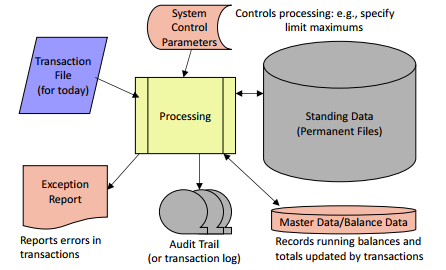
\includegraphics[width=0.7\textwidth]{data_processing}
        \end{center}
        \caption{Data processing}
        \label{fig:data:processing}
\end{figure}

Il processing comprende controllo dei parametri di sistema (es. specificare
minimo e massimo), Standing data (file permanenti), report delle eccezioni
(errori nelle transazioni), log delle transazioni, file delle transazioni
(giornaliero). Una rappresentazione grafica di data processing è riportata
nella Figura~\ref{fig:data:processing}.

\subsection{Processing controls}
I processing controls sono usati per assicurare
l'accuratezza, la completezza e la validità dei dati durante
processing online o batch. Questi controlli sono messi in campo
per verificare che i dati vengano processati solo tramite routine
autorizzate. Esistono due modi per eseguire i processing controls:

\begin{itemize}
\item \textbf{Eseguita transazione per transazione}
\begin{itemize}
\item Editing: il programma testa l'accuratezza, la completezza
e la validità dei dati;
\item Controlli sugli ammontare calcolati: i valori calcolati
sono controllati per essere ragionevoli e non eccedere il massimo;
\item Controlli programmati: software che rileva, logga e inizia
delle azioni correttive per gli errori;
\item Report delle eccezioni: gli errori delle transazioni vengono
riportati con il loro tipo di errore.
\end{itemize}

\item \textbf{Eseguita Batch per Batch}

\begin{itemize}
\item Batch Register: i batch totals sono salvati manualmente per essere
confrontati con i totals di sistema;
\item Run-To-Run Totals: ogni passo del processing riporta i batch
controls calcolati;
\item Reconciliation: un supervisore deve ricontrollare che \emph{tutti}
i dati sono stati salvati e processati correttamente.
\end{itemize}
\end{itemize}


\subsection{Controllo sui file dati}
\begin{itemize}
\item Prerecorded Input: Alcuni campi devono avere dei valori prefissati
quando non si scrive niente. Questo diminuisce il numero di errori;

\item Data File Security: solo l'accesso autorizzato è consentito;
\item Version usage: è sempre usata la versione corretta di un file;
\item Transaction Logs: una traccia per l'audit, salva la data e l'ora
dell'input, l'ID dell'utente, il terminale (su cui è stata effettuata la
transazione) e l'input di transazioni;
\item Before and After Image Reporting: un file contenente dati è salvato
prima e dopo averlo processato. In questo modo è possibile tenere traccia
dell'impatto delle transazioni sui file;
\item Parity Checking: quando un file è inviato, bisogna aggiungere dei codici
per il controllo, per assicurare che sia trasmesso senza errori (hash).
\end{itemize}

Controlli su \textbf{Batch Processing}:
\begin{itemize}
\item
Error reporting \& handing: tutti i report di errori sono stati riconciliati
e le autorizzazioni/correzioni sono state trasmesse in ordine temporale;
\item
One-for-One Checking: i documenti descrivono correttamente il processing
che è avvenuto;
\item
Source document retention: la gestione dei documenti è un'attività molto
onerosa perché richiede che ci sia una organizzazione in piedi;
\item
Internal \& External Labeling: c'è il backup, bisogna etichettarli in
modo da trovare quello giusto.
\end{itemize}





\section{Esercizi}

Gli esercizi sono disponibili in \ref{esCs:ac}

\chapter{Application Audit}
\label{cs:aa}

I compiti dell'auditor includono:
\begin{itemize}
\item Identificare componenti significativi delle applicazioni e
il flusso delle transazioni;
\item Identificare i controlli e valutarne l'efficacia;
\item Testare i controlli;
\item Analizzare i risultati del singolo test per determinare se
il controllo funziona come atteso: così si può giudicare se è inutile,
oneroso, o se è utile, ecc.
\end{itemize}

\section{Strumenti integrati di test}

\begin{figure}[h!]
        \begin{center}
                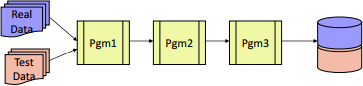
\includegraphics[width=0.7\textwidth]
                {testing_facilities_integrated}
        \end{center}
        \caption[Strumenti integrati di test]{Strumenti integrati di
        test: I dati di test e i dati reali sono fusi.
        Bisogna essere attenti per isolare i dati di test.}
        \label{fig:testing:facilities:integrated}
\end{figure}

\subsection{Operazioni/simulazioni parallele}

I dati vengono processati attraverso due sistemi differenti e i risultati
vengono confrontati.
Questo approccio è utile per verificare nuovi sistemi, comparandoli con quelli
vecchi.

\begin{figure}[h!]
        \begin{center}
                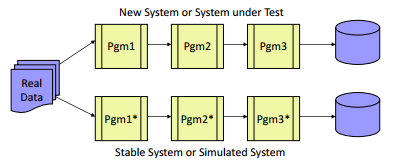
\includegraphics[width=0.7\textwidth]
                {parallel_operation_simulation}
        \end{center}
        \caption{Operazioni o simulazioni parallele.}
        \label{fig:testing:facilities:parallel}
\end{figure}

\textbf{Operazioni parallele:} confrontare il nuovo sistema con quello vecchio
funzionante.

\textbf{Simulazioni parallele:} confrontare il sistema reale e quello simulato.

\subsection{Embedded Audit Data Collection}

        \begin{center}
                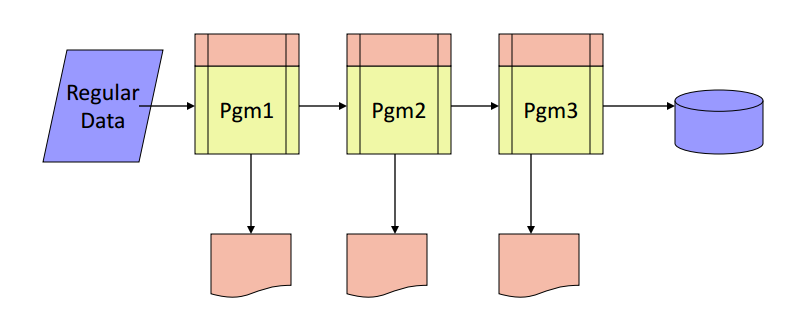
\includegraphics[width=0.8\textwidth]{embedded}
                \captionof{figure}{Embedded Audit Data Collection}
        		\label{fig:testing:embedded:audit:data:collection}
        \end{center}


\textbf{Embedded Audit Modules (EAM):} Il software per l'audit è incorporato
direttamente nei programmi per monitorare specifici tipi di trasformazioni.
Il suo grande svantaggio è quello di rallentare il sistema. Qualora vada tutto
bene sono soldi spesi inutilmente.

\textbf{Systems Control Audit Review File (SCARF):} fornisce informazioni di
tipo statistico riguardo ai file di dati di input "normali", per determinare
per l'auditor se il file è sufficientemente vario.

\textbf{Sample Audit Review File (SARF):} selezionare transazioni random per
fare validazione.

\section{Tecniche di testing per le applicazioni}

\textbf{Test data:}
\begin{itemize}
    \item Test data: testare le transazioni che attraversano programmi reali;
    \item Strumenti di testing integrati: creare delle transazioni di test da
    includere con le transazioni reali;
    \item Programmi di selezione delle transazioni: monitora e seleziona le
    transazioni in input per regolare i cicli di produzione;
    \item Dati di audit incorporati: seleziona transazioni di input random o
    distribuite statisticamente e genera i log durante la produzione.
\end{itemize}

\textbf{Debugging/Processing:}

\begin{itemize}
    \item Mapping: identifica logiche di programmi che non
    sono ancora state testate;
    \item Tracing e tagging: mostra l'insieme delle istruzioni eseguite. Tagga
    con indicatori di luogo le
    transazioni selezionate;
    \item Snapshot: registra flussi di transazioni designate seguendo dei path
    logici.
\end{itemize}

\textbf{Sistemi di validazione:}

\begin{itemize}
    \item Sistema di valutazione base-case: utilizza i test data per testare i
    programmi e verificare che
    le operazioni di sistema siano corrette prima di essere accettate;
    \item Simulazioni parallele;
    \item Operazioni parallele.
\end{itemize}

\section{Tecniche di Auditing Online}

\textbf{Audit Hooks:} sono logiche software integrate nell'applicazione
che stampano dei report, degli errori e dei segnali d'allarme 
quando alcune condizioni particolari sono soddisfatte.
Questo approccio è meno pesante delle EAM perché il controllo 
viene attivato \emph{solo} quando si raggiungono certi path
del \textit{Control Flow Graph} (CFG).

\begin{figure}[h!]
        \begin{center}
                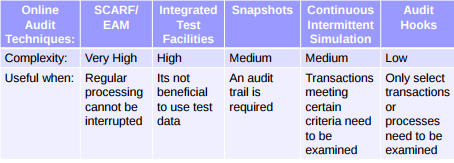
\includegraphics[width=\textwidth]{concurrent_audit_tools}
        \end{center}
        \caption{Strumenti di audit concorrenti.}
        \label{fig:concurrent:audit:tools}
\end{figure}

\noindent \textbf{Auditing online continuo:} permette agli auditor di
testare il sistema senza interrompere le operazioni regolari di una
compagnia.

\section{Esercizi}

Gli esercizi sono disponibili in \ref{esCs:aa}

\part{Incident process e forensics}

Un incidente relativo alla sicurezza può capitare per molti motivi. Un
incidente è catalogato come tale quando c'è una violazione della
\textit{policy} di sicurezza. Un incidente può essere di due tipologie:
\begin{itemize}
\item Malizioso;
\item Casuale (non malizioso).
\end{itemize}

\chapter{Incident Response vs Business Continuity}
\label{IRBC}

Avere un piano di risposta agli incidenti fa parte del \textit{business
continuity plan}.

\section{Business Continuity Plan}

\subsection{Terminologia della recovery}

\begin{itemize}
\item \textbf{Interruption Window:} durata di tempo in cui l'organizzazione
può attendere tra il \textit{Point of Failure} e la riesumazione del servizio;
\item \textbf{Service Delivery Objective (SDO):} livello di servizio in
modalità alternativa;
\item \textbf{Maximum Tolerable Outage:} tempo massimo che si può passare dal
momento in cui si interrompe un servizio al momento di rispristino a pieno
regime.
\end{itemize}

\begin{figure}
        \begin{center}
                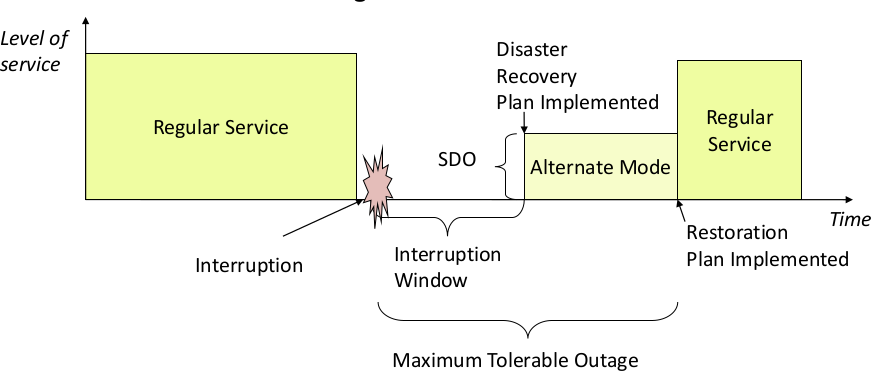
\includegraphics[width=0.75\textwidth]{recovery-times}
        \end{center}
        \caption{Timeline dei tempi di recovery.}
        \label{fig:recovery:timeline}
\end{figure}

\subsubsection{Ruoli}

\paragraph*{Incident Management Team} L'IMT fa parte della \textit{steering
commitee} e sono membri dell'IRT. Sviluppano strategie e piani per la risposta
all'incidente e gestione dei rischi. Ottiene i fondi e verifica le richiesta
di performance e requisiti.

\paragraph*{Incident Response Team} L'IRT è il
team che gestisce l'incidente, ha una conoscenza tecnica dei sistemi e di
``hacking'' (è il classico informatico).

\paragraph*{Investigatore} Presente in aziende grandi, è una persona di fiducia
che ha accesso a tutte le risorse aziendali e si occupa di cercare le cause
dell'incidente che a volte possono anche essere dolose.



\subsection{Incident Response Plan}

Questo piano si suddivide in diversi \textit{step}:
\begin{enumerate}
\item \textbf{Preparazione}: Questa fase è la preparazione dell'incidente,
corrisponde ad una fase di \textbf{analisi dello scenario};

\item \textbf{Identificazione}: Questo step inizia quando si viene
avvisati dell'anomalia e si comincia a cercare la causa del problema.
Più è ricco e complesso il sistema informativo, più è difficile trovare
la causa del problema;

\item \textbf{Contenimento}: In questa fase si cerca di ``limitare i
danni'', con l'obiettivo di mantenere l'operatività. Questo a volte
consiste in  sacrificare elementi della produttività;

\item \textbf{Analisi e eradicazione}: Si cerca di capire cos'è successo
e perché è successo, provando a risolvere la causa;

\item \textbf{Recupero}: Si ritorna con i servizi di nuovo funzionanti,
per ritornare alla fase di preparazione;

\item \textbf{Imparare}:  Questa parte è molto importante, in quanto
imparare la lezione permette di evitare futuri attacchi e di rendere il
sistema più sicuro.

\end{enumerate}

Di seguito ogni passo verrà analizzato in maggiore dettaglio.
